\documentclass[a4paper,11pt,titlepage]{report}

\usepackage[margin=2cm]{geometry}
\usepackage[english]{babel} 
\usepackage{enumerate}

\usepackage{url}
\usepackage{breakurl}
\usepackage{float}
\usepackage{fancyhdr}
\usepackage{graphicx}
\usepackage{listings}
\usepackage{color}

\usepackage[font={small}]{caption}

%LISTINGS PACKAGE SETTINGS 
\usepackage{listings}
\usepackage{color}

\definecolor{dkgreen}{rgb}{0,0.6,0}
\definecolor{gray}{rgb}{0.5,0.5,0.5}
\definecolor{mauve}{rgb}{0.58,0,0.82}

\lstset{ %  
  backgroundcolor=\color{white},  % choose the background color; you must add \usepackage{color} or \usepackage{xcolor}
  basicstyle=\footnotesize,       % the size of the fonts that are used for the code
  breakatwhitespace=false,        % sets if automatic breaks should only happen at whitespace
  breaklines=true,                % sets automatic line breaking
  captionpos=b,                   % sets the caption-position to bottom
  commentstyle=\color{dkgreen},   % comment style
  deletekeywords={...},           % if you want to delete keywords from the given language
  %escapeinside={\%*}{*)},         % if you want to add LaTeX within your code
  %extendedchar=true,              % lets you use non-ASCII characters; for 8-bits encodings only, does not work with UTF-8
%  frame=single,                   % adds a frame around the code
  keywordstyle=\color{blue},      % keyword style
  language=C,                % the language of the code
  morekeywords={*, pid_t, ...},           % if you want to add more keywords to the set
%  numbers=left,                   % where to put the line-numbers; possible values are (none, left, right)
  numbersep=5pt,                  % how far the line-numbers are from the code
  numberstyle=\tiny\color{gray},  % the style that is used for the line-numbers
  rulecolor=\color{black},        % if not set, the frame-color may be changed on line-breaks within not-black text (e.g. comments (green here))
  showspaces=false,               % show spaces everywhere adding particular underscores; it overrides 'showstringspaces'
  showstringspaces=false,         % underline spaces within strings only
  showtabs=false,                 % show tabs within strings adding particular underscores
  stepnumber=2,                   % the step between two line-numbers. If it's 1, each line will be numbered
  stringstyle=\color{mauve},      % string literal style
  tabsize=2,                      % sets default tabsize to 2 spaces
  title=\lstname                  % show the filename of files included with \lstinputlisting; also try caption instead of title
}





%% FANCY HEADER
\pagestyle{fancyplain}
\renewcommand{\chaptermark}[1]{ \markboth{#1}{} }
\renewcommand{\sectionmark}[1]{ \markright{#1}{} }
\lhead{\fancyplain{}{\chaptername \ \thechapter : \ \leftmark}}
\rhead{\fancyplain{}{\rightmark}}


%TITLE 
\title{To be decided\\\Large{--- Individual Research Project ---}}
\author{
       Giuseppe Pes\\
       giuseppe.pes12@doc.ic.ac.uk\\ 
       \small{Supervisor:Prof.\ Cristian Cadar}\\
       \small{Course: XXXX, Imperial College London}
}



\begin{document}



\pagenumbering{roman}
\maketitle

\setcounter{page}{1}

% Thesis Abstract -----------------------------------------------------


%\begin{abstractslong}    %uncommenting this line, gives a different abstract heading
\begin{abstracts}        %this creates the heading for the abstract page

This is where you write your abstract ...


\end{abstracts}
%\end{abstractlongs}


% ----------------------------------------------------------------------


%%% Local Variables: 
%%% mode: latex
%%% TeX-master: "../thesis"
%%% End: 

\setcounter{page}{2}
% Thesis Acknowledgements ------------------------------------------------


%\begin{acknowledgementslong} %uncommenting this line, gives a different acknowledgements heading
\begin{acknowledgements}      %this creates the heading for the acknowlegments


And I would like to acknowledge ...


\end{acknowledgements}
%\end{acknowledgmentslong}

% ------------------------------------------------------------------------

%%% Local Variables: 
%%% mode: latex
%%% TeX-master: "../thesis"
%%% End: 


\tableofcontents
\listoffigures
\lstlistoflistings

\clearpage
\pagenumbering{arabic}

%%% Thesis Introduction --------------------------------------------------
\chapter{Introduction}
Chpter introduction 

\section{System Call interceptor}
%%What’s the problem we are trying to solve? 
%Applications are often vulnerable to buffer overflows, back doors and logic errors which may permit attackers to compromise the application and, depending on the kind of application, they may compromise the entire system. Current operating systems do not provide a sufficient fine-grained mechanism to protect a user from these threats.  The Linux protection model stems from the UNIX one which is based on a discretionary access control DAC, where all programs executed by a user inherit his permission for accessing resources. This model is simple and quite effective, but it is inadequate to the modern operating system because it does not provide any protection against malicious code and flawed.  Several different enhancements have been developed to fill the security gaps in Linux systems, such as SeLinux, LMS (Linux security modules), Audit etc. which offer a more fine-grained control.  However, none of them provide a definitive solution for this problem; rather they address a singular problem, such as? 
%How do we solve it?
%I should introduce the concept of untrusted and trusted software. 
%A widely used approach to improve the operating system security is to confine untrusted code into a controlled environment called sandbox.  The concept of Sandboxing was firstly introduced in [1] as software technique for preventing an untrusted code from escaping its fault domain. They achieved this result by inserting an instruction which set the correct segment of an address before each unsafe instruction.  Nevertheless, this definition is not adapted to describe modern sandbox implemented by using a different technique such as system call interposition. A better and more general definition of sandboxing can be found in [2] as : 
%A technique for creating confined execution environment for running untrusted programs on the same machine.
%One of the core sandbox mechanisms for executing potentially unsafe code is system call interposition. The increment of interest in OS-based intrusion confinement in recent years has brought several new approaches to implement this mechanism.  All these approaches are based on the following observation about attacks: regardless of the nature of an attack, the target system can be compromised only via system calls made by unsafe running processes. It is thus possible to identify and prevent the damage if every system calls made by unsafe processes can be monitored, and launch action to preempt any damage; e.g. abort system call, change its parameters or even terminate the process.
% A system call interceptor is a mechanism which allows a trusted process, which will be called MONITOR, to intercept all system calls made by untrusted process before that the kernel proceeds with executing the system calls. 


%%%NICE 


%NEW INTRDOCUTION
Regardless the nature of an application,resources (such us files,socket, shared memory etc) can be accessed only via the system call interface exposed by the operating system.
The sequence of system calls invoked fully characterised the application's behaviour, that then can be monitored and regulated. \\

A \textbf{system call interceptor} is a powerful technique for investigating all system calls invoked by a program. It usually works by interposing a third agent,called \textit{monitor},between the operating system and the application of interest. This third agent is able to trace and regulate all application's interactions with the operating system.\\


The applicability area of a system call interceptor is rather broad spreading from debugging application such as GDB and auditing (record-replay) to security enhancements (sandboxes,intrusion detection) and virtualisation(UML). In the rest of this section we try to cover all possible applications of a system call interceptor.  

\begin{description}
\item[Debugging] 
\item[Security enhancement]
\item[Virtualisation] 

\end{description}
The first kind of system call interceptor as been introduced for debugging purposes  as tracing routine provided by the operating system. An example of this is ptrace [chapter1]. This tracing routine provides a mean of analysing requested issued by the program in order to help the developer to find a bug in the application. 


Presenting a  detailed analysis of LINUX for the purpose of building interposition tools. 

%Security Purpose 
DETECTION and CONFINAMENT 

There has been a lot of research to improve a system call interception in terms of security and performance because it is the base mechanism for security tools such as sandboxes and introduction detection[ref].The resource control provides by an operating system is usually based on a discretionary access control DAC ( Linux, UNIX-like system) model, where all programs executed by a user inherit his permission for accessing resources. This model is simple and quite effective, though it does not provided any protection against malicious code (back-door) and flaws (buffer overflow). Sandboxing software [ ostia, jailer, sfi, systrace] have been developed to overcome these shortcomings. A sandbox provides a fine-grained control for the resource access by the sandboxed program. These software use a system call interceptor to monitor all system calls made by the sandboxed program and check them against a policies file which constrain a program to a correct behaviour. If one of this policy check fails the system in not executed and the possible malicious action is prevent. 
\\
A system call interceptor is widely used to . 

% 
Introduction detection via analysis of system call traces has received attention throughout recently years [ref]. The problem of a system call tracer is similar to that of a sandboxing tool previously described. The "viewer" is only interested in analysing what calls an application makes in order to find out anomalous system call sequences which may  identify an introduction in the system \cite{introd_detection}. 



%%DEBUG PURPOSE 
As the system call sequence fully characterized the application's behaviour, in the case of an appliation's crash the system call can be reocrder and reproduced that crush in an debugging environment  in order to find out the cause.  [Where is it used] 

%MULTI VERSION CONTROL 
Multi-variant code execution is a run time monitor technique that finds out and prevents malicious code from executing. The idea behind this method is to run two or more slightly different version of the same application in lockstep.At certain synchronization point their behaviour is compared against each other and if a divergence is found, a notification is raised. In multi variant execution,the invocation of a system call is a synchronization point as all variants must make the exact same system call with the same arguments. When one of these attempts to make a system call, this is intercepted by a monitor process that then try to synchronize these with all the different calls within a temporal window \cite{orchestra} + PROF. 


%VIRTUALISATION
A system call interceptor has been successfully used to implement a kernel hypervisor  in \cite{UML_1, UML_2}. UML is a virtualisation technology which enables multiple linux Systems to run as an user application within a normal Linux system. The system call interceptor is used to redirect all system calls made by a program to the guest kernel. This software is used to kernel debugging and for sandboxing application. 

%PORTABLE CODE  
Another interesting application of a system call interceptor is in \cite{CDE}.
CDE creates automatically portable software package using a system call interceptor to track the execution of x86-Linux and collect all data,code and environment required to run it in another Linux machine.  

Why is it important. ? \\ 

Where can it be used ? \\
%record-replay  papers interecept
%sand box thousand of papers 
%introsution dectetion AUDIT	from anom 
%virtualisation  paper SYSM EMU and chinise odule in the kernel
%Portable code GOOGLE 
%Multi version exectuion Orchestra and P

\section{State of art in the system call interceptor}
State of art/different type \\  
% introduce the different way of realizing a system call interceptor 
% ptrace
% kernel enhancement 
% binary rewritting 
% seccomp bpf 
Five different approach may be used to implement a system call interceptor in Linux :
\begin{description}

\item[library]	A library approach was the first used for implementing a system call interceptor [ref]. It relies on the fact that system call are accessed via  wrapper functions, within the glibc library. A system call interceptor can thus be realised by linking the application of interest to a different library which contains an instrumented version of the wrapper functions. This approach has been implemented in \cite{plashglibc}. Its major benefit is that its performance are almost the same as no instrumented application, but it can be easily bypassed invoking directly a system call using low level mechanism.  


\item[Kernel trace tool] The kernel provides features such as ptrace and utrace for tracing and debugging programs. Although this features has been design for debugging purpose, they can be used to successfully build up a system call interceptor in user space without kernel modification (Utrace needs to write a module). 

\item[Binary rewriting]  Binary rewriting consists of modifying the binary program to insert new instructions which allow intercepting the system call made by that modified program. This techniques can be applied both statically as well as dynamically and can be done in a number of different ways, e.g. full binary rewriting, selectively rewriting only sensitive instructions, rewriting only system call instructions.

\item[Seccomp mode-based] mechanisms: is a simple sandboxing mechanism provided by the kernel. It is consist of two system calls seccomp and seccomp-bpf.
 
\item[Kernel enhancement] Following a kernel based implementation, the system call interceptor is implemented within the operating kernel, and all the extension code is executed in kernel mode. A system call interceptor may be inserted modifying the source kernel \cite{Noordende_asecure} or it can be uploaded via a kernel module \cite{Janus}. Both solutions offer the same power in terms what can be accomplished within the extension code, though the later does require neither to compile nor to patch the kernel, it is thus more portable. The kernel approach is exposed in more details in \ref{kernel_mode}.
 



\end{description}

\section{Issues}

conflicts paramenters

\section{Requirements}
So far we have provided a general introduction to all possible mechanisms Linux provided to implement a complete system call interceptor, further all of them will be extended explening how a system call interceptor can be implemented using it, providing real example in which such mechanism has been used.
Which features are needed by a system call interceptor?
A system call interceptor requires a minimum number of capabilities to be effective and thus providing a good base which a sandbox can rely on:
•	Monitor capacity:  A system call interceptor must intercept all attempts to invoke a system call made by the untrusted process before that the system call is executed by the kernel. Furthermore, it also needs to provide a method to analysis the arguments of the system call (and to access to the application’s data space if the real argument is located there) and returned values. This requirement is the core of the intercepting mechanism itself.  
•	Fine-granaid control: we should be able to specify which system call should be intercept and which should be not. Regardless the method used to implement it; a system call interceptor always introduces an overhead with respect to the normal system call’s flow. This greatly improves the performance because we could, for instance, trace the system call which gain access to a new resource but avoid to trace those that use the resource already open.    
•	Preventing the system call execution: when a system call is invoked with unsafe parameters such as open(“/etc/passwd”);. The system call interceptor must have a means of aborting its execution without aborting the entire process and setting a proper return value i.g. EPERM. 
•	Monitoring all children:  The system call interceptor must intercept and monitor all children of the traced processor. It is crucial that the children of a sandboxed process must be constrained to the father's policy rules.
•	Dealing with multithread application: another important requirement it the possibility to trace all threads of the traced application efficiently, without stopping them if not necessary. 
Why characteristics should a System call interceptor have? 


\section{Design goal} 
-flexibility 
-compatibility 
-security
-deployability
-performance

-Security 
-realiability 
-sdfd
Robustness : the capability, in case the tracer process crashes unexpectedly to terminate all the traced processes.  
Principle of Least Privilege: 	 if the monitor is compromise the attack gains only the user priveldge and not the root. 
All of these of this techinique introduce an overhead in the normal computation, so we have to use a method to assess thei performance and/ ///
. In this document we will introduce a detail analysis of Linux for the purpose of building interposition mechanisms. 
Which resource must be protected? 
	File system
	Network access 

QUESTION :  
1	Problem ?
2	Sand box 
3	What is a system call interceptor.
	< security, portability, configurability.>
4	How can we asses them? How can we compare them?
A fault domain is a set of hardware components – computers, switches, and more – that share a single point of failure


Design GOAL  \\
% 

Issues. \\ 
% the proble which affects a system call interceptor 
% papers for this. 
OVERHEAD 

Remain Document structure  \\ 
% introduce the different part of the document 

 ----------------------------------------------------------------------
%%% Local Variables: 
%%% mode: latex
%%% TeX-master: "../thesis"
%%% End: 

%PTRACE CHAPTER 
\chapter{Ptrace}

Like most of the UNIX-like operating systems, Linux supports the \textbf{ptrace} system-call interface. Ptrace provides a means by which a process might observe and control the execution of another process; the first process is referred to as the \textit{tracer} process and the latter as the \textit{tracee} process. Since its introduction in the Linux kernel version 1.0,  ptrace has been mainly employed in implementing debuggers, such as GDB and DBX, where it is used to insert breakpoints into the running program; and for system-call tracing. For example, the command strace exploits ptrace requests to retrieve information regarding the system-calls invoked by a program. 

The ptrace's interface is:
%I use the center environment in order to have the same space 
%between the previous and the next text section.
\begin{center}
\lstset{escapechar=@,style=c}
\begin{lstlisting}[caption={Synopsis ptrace system call}]
					long ptrace ( enum __ptrace_request request, pid_t pid, void *addr, void *data)
\end{lstlisting}
\end{center}

Ptrace supports numerous different type of actions, for a comprehensive list see  \cite{ptrace}, though the most representative ones are:

\begin{itemize}
\item Attach to, or detach from the process being traced (the tracee), used to install the tracing mechanism.  
\item Read and write the tracee's memory and its status registers.
\item Signal injection and suppression.
\item Resume the execution of the tracee allowing it to continue until 
	  an event of interest occurs (e.g. a system-call is invoked).
\end{itemize} 

%WHEN A PROCESS CAN ATTACH TO ANOTHER PROCESS
The tracer process gains extensive control over the operations of the tracee process. This includes manipulation of its file descriptors, memory, and registers. It can single-step through the tracee's code, observe and intercept system calls and their results. Furthermore, it can manipulate the tracee's signal handlers and both receive and send signals on its behalf. While a process is being traced, all events such as attempting to invoke a system call or receiving a signal are turned into a  \ci{SIGCHLD} \footnote{The communication between the tracee and the tracer is performed using the standard UNIX parent/child signaling over \emph{waitpid} system call}  signals that are delivered to the tracer process. Every time the tracee receives a signal, it is stopped so that the tracer may analyses its status and if necessary changes its execution. 


Although ptrace has been primarily designed for debugging purposes, it offers enough flexibility to be used for different tasks as well. It has been successfully and widely used to implement a \emph{user-space system call interceptor} in \cite{Provos02improvinghost,Janus,MapBox, Noordende_asecure, Jain99user-levelinfrastructure}, though it entails numerous limitations. The major disadvantage of the ptrace approach is that the performance may be remarkably reduced in a program which uses intensively system-calls. Several context switches between kernel space and user space are introduced respect to a non-traced execution to support the tracing mechanism. However, an interceptor mechanism can be employed in different contexts and therefore different criteria can be used for choosing it. For example, when performance is not a fundamental requirement such as for debugging, ptrace offers a valid solution. 

One of the most important feature offered by a system-call interceptor is the possibility of retrieving the system call number and its arguments. This may be used in applications for auditing purposes such as \emph{strace} \cite{strace}, where all system calls and their arguments are recorded or sandbox application \cite{Provos02improvinghost,Janus} where each system call is tested against a policy specifying which arguments are allowed and which are not.

Ptrace provides the possibility of retrieving both system call number and its parameters by accessing the status registers and the space memory of the tracee. Accessing the tracee's memory via ptrace is actually rather inefficient as ptrace permits only to pass a small fixed-size block  between the two process. This is one the crucial limitations of ptrace and different techniques have been developed during the recent years to mitigate it. These are presented in the \ref{memory_access} section. 


Another requirement missed by ptrace is to support multi-thread applications. Ptrace actions are specified for single thread via its ID, thus in a multithread application each of its threads must be attached individually. This action if not handled carefully might leave open a temporal window during which some system-calls might not be intercepted. The section  \ref{multi_thread_application} surveys different problems regarding tracing multithread application and provides an effective solution to them.
An important requirement for an application such as a sandbox is the possibility to deny the execution of a system call when it does not satisfy the policy. While other operating system, such Solaris provide a way of aborting a system call, ptrace does not offer any.  

In the section \ref{aborting_systemcall} different methods to overcome this shortcoming are introduced.Finally, another requirement missed by ptrace is the possibility to trace only a subset of the system calls provided by the operating system and leave others to be executed without any overhead. This reduces the tracing overhead in several different cases, for example, in a sandbox application  where only the system calls which might affect the security of the operating system should be intercepted. In \cite{Noordende_asecure} all system calls which open or change a file descriptor (\ci{open}, \ci{socket}, \ci{bind}) are intercepted, while those which use it (e.g. \ci{read}, \ci{lseek}, \ci{write}) are not. 


Ptrace has been used also for virtualising system calls in \cite{UML_1,goanna, UML_2}. In this case all system-calls invoked by the tracee must be nullified in the host architecture in order to be virtualized; see section \ref{aborting_systemcall}. The ability to write into the tracee's memory allows the tracer to change also the tracee own code segment. This feature has been exploited by specialised programs to patch running programs in order to avoid  bugs or to fix security lacks. 

Although its limitations and shortcoming ptrace is the standard tracing mechanism used in Linux and Unix-like operating system. This success is due principally to two factors. 
The first is that ptrace provides an easy way to set up the tracing mechanism in user space compared with other approach such us kernel-based tracing mechanism. It can be used without root privilege, provided the tracer has enough privilege to trace the process of interest. Secondly, even though ptrace is not a POSIX system call, it allows for the interception infrastructure to be easily ported between different operating systems.  The remainder of the chapter introduces how to set up a system call interception using ptrace section \ref{Ptrace_tracing_mechanism} and how to overcome the shortcomings and limitations discussed before. 


\section{Ptrace tracing mechanism}
\label{Ptrace_tracing_mechanism}

Ptrace may be successfully used to build an effective system call interceptor, ensuring that the tracer process intercepts all system call made by the tracee process and its child processes. This section exposes in details how to implement a system call interceptor using ptrace. 

There are two different ways to install the tracing mechanism. The tracer might invoke the fork system call to create a child process which notifies the kernel its willingness to be traced by calling ptrace with the argument \ci{PTRACE_TRACEME}. This request causes the kernel to set a trace flag (\ci{PT_TRACED}) in the target process descriptor and stop it by setting its state to non-interruptible sleep. This approach is usually used before the tracing software initiates a new program by invoking \ci{exec} system call. Alternatively, the monitor process can make a request to the kernel for tracing a running process via ptrace specifying the argument \ci{PTRACE_ATTACH} and the target process pid. In this case, there are three conditions to be checked:
\begin{enumerate}
\item If the privileges of the tracer process allow it to trace the tracee process. Ptrace can attach only to processes that the owner can send signals to (typically only their own processes).
\item If the tracee process is being already traced.
\item If the target process belongs to a set of process that cannot be traced (init and itself).
\end{enumerate}

If all previous controls are satisfied, the monitor process becomes the parent of the traced process and the trace flag is set on its process descriptor. Then, as the previous case, the tracee is put in a non-interruptible sleep state by a \ci{SIGSTOP} signal sent automatically by the kernel. This signal in fact kicks off the tracing mechanism, but it has been seen as possible source of security issues as a process should not be aware of being traced \cite{ptrace_seize}. In order to overcome this shortcoming the \ci{PTRACE_SEIZE} and \ci{PTRACE_INTERUPT} requests have been introduced in the 3.4 kernel version. \ci{PTRACE_SEIZE} attaches the process specified in the pid to the process that has issued the request. Unlike \ci{PTRACE_ATTACH}, \ci{PTRACE_SEIZE} does not stop the process. To stop a process traced using it, an \ci{PTRACE_INTERRUPT} request need to be issued. This cause the stop of the process without sending a \ci{SIGSTOP} signal, making all the tracing process transparent to the tracee. 
The possibility of attaching a running process is particularly useful when a process, which has been created by a different process from the tracer, has to be monitored. A typical example of this situation is when a tracee spawns a new thread. The newly thread must be attached using one of the previous requests as the trace flag is not inherited.  

%% %%% VIRTUAL PARENT `	
It is worth noticing that in both cases the tracer becomes the parent of the tracee process. The \ci{task_struct} of a Linux process has two fields:
\begin{center}
\lstset{escapechar=@,style=c}
\begin{lstlisting}[caption={ Parent and real parent fields with task\_struct Linux}]
		struct task_struct *real_parent;	/* real parent process */
		struct task_struct *parent;				/* recipient of SIGCHLD, wait4() reports */
\end{lstlisting}
\end{center}
Usually both field point to the process which has created the current process. When a process is being traced the parent field is modified in order to point to the tracer process which becomes the parent of the child process for most purposes (e.g. it will receive notification of  child  events  and  appears  in \ci{ps}  output  as  the  child's parent), while the real parent remains the original one as invoking \ci{getpid} the pid of the original process is retrieved. In Linux a process has exactly one process father. Consequentially, this limits ptrace to track only one process per time making it a no-efficient mechanism for tracing multithread applications. 
%%%%%%%%%%%%%


When the tracing mechanism has been correctly started, all system calls made by the tracee are intercepted by the tracer. The tracee process is put in a stopped state by the kernel each time it receives a signal or attempts to invoke a system call.  Once the tracee has been stopped, the tracer is notified via a signal \ci{SIGCHILD} and then it is allowed to access the tracee address space.  The tracer may handle this signal either through a wait-family system call or by installing a dedicated handler. 
In the case of system call interceptor, the only relevant notifications are those regarding the attempt of invoking a system call. Precisely, the tracer should be notified twice, at the entry point before the system call is executed and at the exit point before the traced process is resumed. The sequence of events triggered when the traced process invokes a system call is depicted in Figure  \ref{fig:ptrace_systemCall}.

%FIGURE 
\begin{figure}[h]
\centering
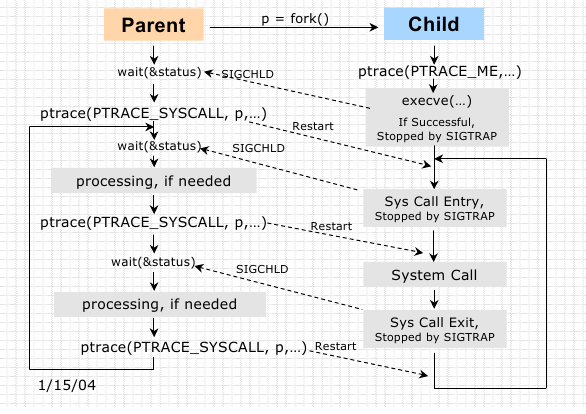
\includegraphics[scale=0.6]{Chapter1/Chapter1Figs/ptrace_systemcall.png} 
\caption{System Call invocation}
\label{fig:ptrace_systemCall}
\end{figure}


The cause of the stop in the tracee can be identified through the status variable returned by the wait primitive or the integer argument in the handler function.  The Linux signal library  provides different macros to easily deal with this signal status variable. The cause that determines the stop of the tracee process can be retrieved as follows:
%Not good we want to identify only system entry adn system exit 
\begin{center}
\lstset{escapechar=@,style=c}
\begin{lstlisting}[caption={Condition that identifies SIGTRAP signals}]
									WSTOPSIG(status) & (WIFSTOPPED(status) == SIGTRAP)
\end{lstlisting}
\end{center}

Unfortunately, the status variable will assume the same value also when a SIGTRAP signal is delivered to the tracee for a different reason from invoking a system call. \\
This ambiguity may be solved in two different ways. Further information about the source of the signal might be retrieved by issuing a ptrace request with \ci{PTRACE_GETSIGINFO}.  Although this will introduce a further system call for each \ci{SIGTRAP} signal delivered to the trace, which in the case of a traced process are the most common.  This performance decrease can be avoided using ptrace with the \ci{PTRACE_O_TRACESYSGOOD} option. This option ensures that when a signal trap is generated because the tracee is trying to make a system call the 7th bit of signal status is set.

\begin{center}
\lstset{escapechar=@,style=c}
\begin{lstlisting}[caption={Condition that identifies exclusively system call entry and exit}]
									WSTOPSIG(status) & ( WIFSTOPPED(status)== SIGTRAP | 0x80)
\end{lstlisting}
\end{center}

Now, the tracer can skip all false notifications and analyse only those regarding a system call. 

%PARAMATER ACCESS
One of the most important feature of system call interceptor is the possibility of identifying the system call invoked by a process and retrieve all its arguments. The convention adopted in Linux \ref{system_V_abi} for calling a system call is to insert the number of the system call into the \ci{EAX} register for x86\_32 architecture and in the \ci{RAX} register in x64, along with its parameters. The maximum number of system call parameters is 6 so the stack is not involved in passing arguments. The table below resumes the role of some registers during a system call invocation for both x86\_32 and x64 architecture, these structures can be found in \emph{sys/user.h}. 

\begin{multicols}{2}

\begin{center}
\lstset{escapechar=@,style=c}
\begin{lstlisting}[caption={Linux structures representing the general purpose registers of x64 CPU}]
/* x64 architecture */				
struct user_regs_struct				
{                                 
  ....                                         
unsigned long int rdi; /* 1th parameter */
unsigned long int rsi; /* 2th parameter */		
unsigned long int rdx; /* 3th parameter */       
unsigned long int rcx; /* 4th parameter */   
unsigned long int r9;  /* 5th parameter */     		
unsigned long int r8;  /* 6th parameter */   
unsigned long int rax;  
/* System Call number */
unsigned long int orig_rax;			   
unsigned long int eflags;            
 ....   
};                                 
\end{lstlisting}
\end{center}

\begin{center}
\lstset{escapechar=@,style=c}
\begin{lstlisting}[caption={Linux structure representing the general purpose registers of x32 CPU}]
/* x32 architecture */				                                
 struct user_regs_struct
{
  .....
  long int ebx;	 /* 1th parameter */
  long int ecx;  /* 2th parameter */
  long int edx;  /* 3th parameter */
  long int esi;  /* 4th parameter */
  long int edi;  /* 5th parameter */
  long int ebp;  /* 6th parameter */
  long int eax;
  /* System Call number */
  long int orig_eax; 
  long int eflags;
  .... 
};                                 
\end{lstlisting}
\end{center}
\end{multicols}

 
While the tracee process is in stopped, the tracer can retrieve and modify the values of the tracee processor register via \ci{PTRACE_GETREGS/PTRACE_SETREGS}. However, this methods offers only a way to access to the direct parameters that are within the registers. To retrieve the value of the indirect parameters whose address is contained in the resister, the tracee memory needs to be accessed. The tracee memory is accessed, before the system call is executed, to retrieve the system call identifier and arguments. This is used in software such as sandbox, for example, \cite{Provos02improvinghost,Janus,MapBox, Noordende_asecure} to check whether the system call invocation satisfies the requirements specified in a policy file or for auditing purposes in \cite{strace}. Furthermore, there is also the possibility to access the tracee memory when the process is stopped after the execution of the system call. This gives a means of analysing the system call return value, which is important for applying post policy rules in a sandbox application. Post policy rules are used for those system call where a sensitive value is known only after the call is executed such as \ci{accpet}, \ci{recv}. Accessing the memory always introduces an overhead which has to be taken in account when performance is an important aspect of the application. Ptrace offers different type of requests \cite{ptrace} to accomplish this, however all of them are limited in bandwidth to 4 bytes in x86\_32 architecture and 8 bytes in x64. Different approaches for accessing the memory of the tracee process are discussed in detail in \ref{memory_access}. 

Once the control over the system call arguments are terminated, the tracee's execution is to be resumed. Ptrace provides for the tracer the ability to fully control the execution of the tracee. The execution of the tracee can be resumed via one of the following ptrace requests:

\begin{description}
\item[PTRACE\_SYSCALL] continues execution until next entry or exit from a system call.
\item[PTRACE\_CONTINUE]continues execution until the tracee receives a signal.
\item[PTRACE\_SINGLESTEP] continues execution until the next tracee instruction. 
\end{description}

As we are only interested in intercepting a system-calls the execution of a tracee is resumed by calling ptrace with \ci{SYS_SYSCALL} as argument, its execution continuing until the next system call event. 



\section{System call virtualization}
\label{system_call_virtualization}
%Virtualization has become increasingly popular and a new demand for Linux is to act as a hypervisor. Different virtualization technologies have been developed to cope this increasing demand, such as instruction emulators QEMU, full or partial hardware emulation. 
 
System call virtualization is a technique to emulate the execution of a system call made by a process. Ptrace can be used to set up a system call virtualization mechanism in Linux. This approach has been followed by Jeff Dikk \cite{UML_1, UML_2} developing \textit{User Mode Linux} (UML) whose goals was to run Linux kernel in user space for easing the debugging of kernel. 

A system call virtualisation needs a way to nullify system calls so that they would execute in such way as to cause no effects on the host.  However, ptrace did not provide a means of aborting a system call. This shortcoming has been fixed introducing the possibility to change the actual system call. Annulling a system call can be done by substituting the actual system call with a a call \ci{getpid}, which introduces a small overhead due to its execution. 
When a system call is virtualised, there is no need to intercept the exit point because the system call has been nullified.  This prevents the execution of two context switches between kernel space and user space which yields to a 50\% improvement in the performance. These ptrace enhancements have been introduced in the kernel mainline and they can be used by calling ptrace with the parameter \ci{SYSEMU} \cite{ptrace}. As it has already been said, this prevents the system call to be executed and notifies the tracing parent only at system call entry.  
The tracing mechanism can be installed in a similar manner has described in the previous chapter. The only difference is that when the traced software is resumed issuing ptrace with \ci{PTRACE\_SYSEMU} parameter instead of \ci{PTRACE\_SYSCALL}. 
System call virtualization is implemented by the tracing thread intercepting and redirecting process system calls to the system call handler.  It reads out the system call and its arguments, then annuls this in the host kernel and executes the virtual system call instead. When the emulated system call is finished; the return values are stored in the memory of the traced process.

An example of this approach can be found in \cite{goanna}, where ptrace has been used to create a user-level file system development environment.  The bulk of the application consists of a monitor called GOANA which intercepts all system calls made by the traced process. Once the system call has been intercepted this is substituted with a prototype function.  This provides an easy way to test a file system prototype because we do not need to deal with massive body of kernel-level code and  due to the fact it runs on user space the system can be analysed using a powerful debugger such as GDB which would have been impossible to use in kernel mode. 
The performance is still the main problem of this approach as well.   Even though by using \ci{SYSEMU} the context switch between user space and kernel space are reduced to 2. There is still the necessity  to access the memory at the system call entry point to retrieve its arguments and after the execution of the system call is finished to store the return values. This is a critical part of each monitor process, this problem as in the previous case will be treat in detail in the next section. \\


%%%%%%%%%%%%%%%%%%%%%%%%%%%%%%%%%%%%%%%%%%%%%%%%%%%%%%%%%%%%%%%%%%%%%%%%%  MEMORY ACCESSS %%%%%%%%%%%%%%%%%%%%%%%%%%%%%%%%%%%%%%%%%%%%%%%%%%%%%%%%%%%%%%%%%%%%%%%%%%%%
\section{Memory access}
\label{memory_access}

The tracer process is executed in user mode, it thus is not allowed to write or read the memory space of the tracee process. The tracer needs to read the memory of the tracee process in order to retrieve the contents of the indirect parameters such as strings or pointers.
There are two kinds of arguments direct and indirect, the former is contained in the general purpose register, while the latter is contained in the process memory and its address can be found into registers. The maximum argument number for a system call is six, so they fit in the register and there is no need to access the process stack.Also, the monitor needs to write the target memory address, for instance, when the system call is emulated and the outcome of the computation need to be stored in the traced memory space.\\

\textbf{Ptrace}\\
One method to access the memory of the tracee process is provided by ptrace. The monitor process may read from the monitor process calling ptrace with \ci{PTRACE_PEEKDATA} when the target process is suspended. The writing procedure can be performed in a similar manner by using \ci{PTRACE\_POKEDATA}. Unfortunately, ptrace transfers only 4 bytes per time in x86\_x32, and 8 byte in x64, therefore it has to be called many times to read or write a large amount of memory. Every call to ptrace requires a context switch from the monitor to the kernel and back, which decreases its performance since to make it, in fact, not a feasible way with a large amount of data. The Linsting \ref{ptrace:mem} is an example of using ptrace to retrieve a buffer from the tracee space memory. In order to improve the performance in accessing the traced memory space different approach can be taken. 
\begin{center}
\lstset{escapechar=@,style=c}
\begin{lstlisting}[label=ptrace:mem, caption={Function which retrieve a buffer of size count from the tracee memory. Note, the value retrivied by a single ptrace call has to be converted to the char type before being inserted in the buffer. }]
void peek_data_ptrace (pid_t tracee, const void * source, size_t count, void * dest) {
    
  unsigned long int value=0; 
  char stringValue[DWORD_SIZE]; 
  int i=0, 
      chunks=count/DWORD_SIZE; 
  
   if (count%DWORD_SIZE) 
      chunks++; 
      
  for (i=0; i < chunks; i++)   {
  
    if((value=ptrace(PTRACE_PEEKDATA, tracee, source + (i* DWORD_SIZE), NULL)) < 0) {
     perror("Ptrace PTRACE_PEEKDATA"); 
     exit(1); 
   }
   convert_intToChar(value, stringValue);
   memcpy(dest + (i* DWORD_SIZE), stringValue, DWORD_SIZE); 
  }
  
}
\end{lstlisting}
\end{center}


\textbf{Shared Memory}\\
The monitor process has to ensure that the target process can access to the shared memory. In Jailer \cite{Noordende_asecure} the shared memory is set up using a pre-load library technique. The pre-load library uses \ci{mmap} to read-only map the memory region in the target’s process space, in addition, it loads some code routine. Another technique presented in \cite{orchestra} consists of replacing the first system call made by the target process with an appropriate one such as \ci{shmget}, \ci{ipc} after making a backup of the values contained in the registers. This makes the target to run the new syst em call and attaching the shared memory to the target process. After performing this operation, the original system call is restored by using the register values previously saved.  In both cases a small code is injected to the space memory which copies the content of a buffer to another one. When the monitor process needs to access to an indirect arguments, it can retrieve the base address from the registers by using ptrace and then use this routine to copy all the buffer in the share memory. In the Jailer system, the values of registers are modified to point to this memory area for security reasons  \cite{garfinkel:traps}.\\

\textbf{FIFO}\\
Another approach proposed in \cite{orchestra} is to use FIFO structures.  FIFO is inter-process communication which allows the monitor process to communicate to the target process by writing to and reading from the FIFO.  The pipe can be created using the system call \ci{mkfifo} and then it can be managed via I/O system calls usually used to deal with files (in fact the FIFO is a file in the file system). 
The target process can easily open the FIFO by using the FIFO’s name as parameters calling open.  While, if the target process has been spawned by the monitor process, it inheritances the file descriptor corresponding to the FIFO open by monitor process. However, there is still need to use a routine to copy the values from the target process space to the pipe.  Other ipc mechanisms such message queue \cite{Noordende_asecure} can be used in a similar fashion. \\

\textbf{ Using /proc interface} \\
The proc file system is a pseudo-file system which is used as an interface to kernel data structures. This interface may be used to collect information regarding the execution of a program such as file descriptors, memory layout and so on. Two files within this hierarchical file system are particular relevant for the purpose of accessing the memory of a traced processed. The first is \ci{/proc/pid/maps} which contains a list of all the memory regions and their access permissions currently mapped in the address space of the process identified by the pid within the path. This feature is used to retrieve the location of shared libraries or shared segment within the address space of a process. It also used to identify whether the process is using a \ci{xVSDO} mechanism to boost up the process of invoking a system call. The other file of interest is \ci{/proc/pid/mem}, it has been introduced to provide an alternative to the ptrace approach discussed before. This file can be used to access the pages of a process's memory via the classic system call  \footnote{The classic system calls used to handle files in Linux are open, lseek, read, write, close} used to deal with files. The Listing \ref{proc:mem} presents a possible way to implement this approach. Some constrains must be respected by the process that wants to access the memory of another process using this method.
\begin{itemize}
\item  The process that wants to read from or write to \ci{/proc/pid/mem} must trace the execution of the process identified by the pid via ptrace.
\item  The tracee must be in a stopped state.  
\end{itemize} 
If the previous checks are not respected an \ci{ESRCH} error is retrieved. A cautious approach should be taken using this method as the ability of writing to the process's memory might be disable in some kernel versions. This is due to the confusion caused by the introduction of a vulnerability when the writing ability was first activated. The writing function within the kernel performed a poor permission check which could be exploited by a user to gain root privilege \cite{mem_vul}. However, a recent kernel (after 3.0) should be bug-free and support the writing function. 

\begin{center}
\lstset{escapechar=@,style=c}
\begin{lstlisting}[label=proc:mem, caption={Function which retrieve a buffer of size count from the tracee memory using the proc interface. }]
void peek_data_proc (pid_t tracee, const void * source, size_t count, void * dest){

  char mem_file_name[100]={0};
  int mem_fd; 
  
  sprintf(mem_file_name, "/proc/%d/mem", tracee);
  // No need to open and close the file each time the tracee memory is accessed 
  mem_fd = open(mem_file_name, O_RDONLY);
  lseek(mem_fd, (__off_t)source, SEEK_SET);
  read(mem_fd, dest, count);
  close(mem_fd); 
  
  return;
}
\end{lstlisting}
\end{center}

 
\textbf{Cross memory attach}\\
The space memory of a running process can be also accessed using \emph{cross memory attach}, a new mechanism that has been recently introduced in the Linux kernel
 \ref{cross_memory_attach}. This mechanism is implement by two new system calls \cite{cross_memory_attach_syscall} that transfer data between the address space of the calling process and the process identified by pid.  The data moves directly between the address spaces of the two processes, without passing through kernel space improving the performance respect to the previous  approach. This has been successfully employed in \cite{mx:icse13} to access the system call's parameters. Listing \ref{cross:mem} shows how to use these new function to gain a fast access to the tracee's memory. For obvious security reasons, there are some restrictions that a process must respect in order to access the memory of another process. In order to perform the copy both process must have the same ownership or the calling process must have the \ci{CAP_SYS_PTRACE} capability. The permission required is exactly the same as that required to perform a ptrace attach to another process. 

\begin{center}
\lstset{escapechar=@,style=c}
\begin{lstlisting}[label=cross:mem, caption={Function which retrieve a buffer of size count from the tracee memory using cross memory attach method. }]
void peek_data_cross (pid_t tracee, const void * source, size_t count, void * dest){
  
  struct iovec remote[1], local[1]; 
  ssize_t bytes_counter; 

  local[0].iov_base = dest;
  local[0].iov_len = count;
  
  remote[0].iov_base = (void *) source;
  remote[0].iov_len = count;

  bytes_counter=process_vm_readv(tracee, local,	 1,	 remote,	 1,		 0);

  if ( bytes_counter < 0 ) {
    perror("Vm_read"); 
    exit(1); 
  }
  
}
\end{lstlisting}
\end{center}


\section{Multi thread applications}
\label{multi_thread_application}

 
Nowadays, most the applications are multithread.\footnote{In this chapter, the term multithread process/application refers to an application/process whose threads have been created using the system call \emph{clone} \cite{clone} with the \ci{CLONE_THREAD} flag.} For example, a web server usually creates a new thread for each incoming request and let this newly created thread to accomplish it. This family of applications must be taken into account as possible target process for a system call interceptor and this requires a thoroughly analysis. As we already said in the introduction part, one of the most import requirements of a system call interceptor is to provide a means of intercepting all processes spawned by the traced process. Ptrace misses this aspect because it provides a tracing mechanism for single thread \cite{ptrace}; where each thread must be attached individually to the tracer process issuing a request with \ci{PTRACE_ATTACH}. Moreover, a child process does not inherit the trace flag from the parent, so it can run untraced until the father attaches to it. These flaws make tracking multithreaded application difficult and error prone \cite{garfinkel:traps}, so that some applications \cite{Noordende_asecure} decided to not support this kind of applications.

Nevertheless, ptrace offers a solution, though it is quite elementary. By setting the option \ci{PTRACE\_O\_TRACECLONE}, the tracee will be stopped at the next \ci{clone} function and the tracer will start tracing the newly cloned process.  This solution, in fact, is not a feasible way to trace multithread application when performance is important because each time a signal is delivered to a traced thread, all threads in the traced poll enter in a stop state. 
This introduces an unnecessary latency because the other threads (those that have not received any signal) must wait until the event is processed by the tracer and the entire application is resumed before being able to continue their tasks. However, in application where performance is not important, for instance debuggers, this represents a valid solution. In fact, this approach is used by GDB.  Another issue related with this approach is that ptrace does not always guarantee that the forked processes are always automatically traced.  Linux allows setting a flag on \ci{clone} (\ci{CLONE_UNTRACED}), which determines whether the child process can be traced or not. However, this can be easily solved noticing that the clone function will be intercepted by the monitor program and it can modify its arguments changing that flag to \ci{CLONE_PTRACE} which makes the process traceable.\\ 
The common approach to deal with multithread application is to create a new tracer process \cite{Jain99user-levelinfrastructure, Noordende_asecure, orchestra,strace, Provos02improvinghost} for each new tracee process. Unfortunately, this solution arises a race condition which might yield to some system calls to escape from being intercepted. The new monitor is not allowed to trace the newly thread until the parent monitor detaches from it.  When the parent monitors detaches from it the kernel sends a message to the tracee process and allows it to continue its execution.  This leaves a small temporal window within some system calls might escape.  This is critical problem in application in software such as sandbox, where all system calls must be intercepted for obvious security reason. A completely different approach is taken by \emph{strace} where this problem is not tackled because a missed system will not comprise the entire application, while solving it will complicate the code, and the temporal window is rather small and the probability of missing a system call or more should be quite low.

A possible kernel enhancement, which solves this, would be to notify to the tracer when the newly thread has been created but it is not yet running. This would give the opportunity to safely attach a new tracer to the newly created thread without losing any call. Instead the tracer receives a tracing event only on the child’s subsequent system call.

This problem has been addressed successfully in \cite{orchestra} as follows.  When the tracee process spawns a new thread, automatically it is stopped by the kernel and the monitor start monitoring the newly created thread. At its first system call invocation, the monitor makes a backup of all new tracee process registers and then it substitutes the requested system call with a \ci{pause} system call and finally lets it continue its execution.  When the new process is resumed, it will enter in a pause state due to the injected system call. While this process is in the sleep state, the monitor is allowed to detach from it and the new monitor can safely attach to it. Once the new monitor has successfully attached, it restores the previous system call so that the execution of the new tracee process can continue, ensuring that the original application's behaviour is preserved. Although this solution works well, it introduces a small time overhead due to the execution of the pause system.  Moreover, a communication between the new monitor and its father is needed to retrieve the backup information regarding the execution context of the new thread in order to restore the previous system call. 

This problem has been recently solved in Linux kernel 3.5, using ptrace together with a seccomp-bpf filter. A BPF filter can be set up to translate each system call request to a signal to the tracer process. The key advantage of seccomp-BPF filters  is that, they are inherited by the child processes. Therefore, the child processes can be safely traced using seccom-bpf mode with a tracing filter. This method has also the advantage of avoiding to overcomplicate the implementation code. The seccomp-bpf filter are discussed in \ref{filter}. 

\section{Aborting a system call}
\label{aborting_systemcall}

Having the possibility to abort a system call is an important feature. Let’s consider the following scenario. A large application such as database has been sandboxed for security reason. It is possible that due to the nature of the application and the high number of system call requests, some policy checks fail. When this happen the system call should be nullified, but if this feature is not provided the only solution is to terminate the application even if there is not any real threat.
Unfortunately Linux doesn't provide any means of aborting a system call.  This lack has been one of the main reason because ptrace was not considerate a feasible way to implement a system call interceptor in Janus version 1 \cite{Janus}. 
Different solutions have been propose \cite{Jain99user-levelinfrastructure, goanna}, but this problem has been solved by Jeff Dikk who has implemented a patch for the Linux kernel. This patch allows the tracer to substitute the invoked system call with another one by inserting a different system call id in the \ci{EAX} register for x86\_32 or \ci{RAX} for x64. Leveraging on the enhancement introduced for UML, the tracee’s system call can be substituted with the low-overhead system call \ci{getpid}.
This technique for aborting a system call raises another problem, which value should be returned? \\
One possibility is \ci{EINTR} which represent the error code for system call interrupted. However, this is not a good choice because some application may be coded in such a way that, if they receive \ci{EINTR} error they will retry the system call. If this happens in a loop the application gets stuck and the only way to break that loop is to kill the entire application. A better error code is \ci{EPERM}, which stands for operation not permitted.
\chapter{Kernel-based tracing mechanisms}
\label{kernel_mode}

Kernel tracing mechanisms were originally developed in response to the limitations of the existing tracing mechanisms such as ptrace. Since the early 2000, several sandbox tools have been developed using a system call interceptor implemented within the kernel \cite{Janus,Noordende_asecure,Provos02improvinghost,Garfinkel03ostia:a} either using a kernel enhancement (ptrace++) or a kernel module (mod\_janus).

%%%%%%%%%%%%%%%%%%%%%%%%%%%%%%%%%%%%%%%%%%%%%%%%%%%%%% KERNEL MODIFICATION %%%%%%%%%%%%%%%%%%%%%%%%%%%%%%%%%%%%%%%%%%%%%%%%%%%%%%%%%%%%%%%%
Two different approaches can be taken to develop a system call interceptor in the Linux kernel. As the source of the kernel is available, a completely new tracing infrastructure might be introduced in the kernel exposing its tracing functionalities to user space as in the case of \textit{ptrace} or at kernel space as in the case of\textit{utrace}. This approach requires a massive change in the kernel source that is difficult to implement and error-prone due to the complexity of the kernel. Furthermore, it is not a portable solution as it will not be inserted into the Linux source (see case utrace),and thus it should be dispatched as kernel patch which is not easy to install and require to compile the entire kernel. 

%%%%%%%%%%%%%%%%%%%%%%%%%%%%%%%%%%%%%%%%%%%%%%%%%%%%%% KERNEL MODULE %%%%%%%%%%%%%%%%%%%%%%%%%%%%%%%%%%%%%%%%%%%%%%%%%%%%%%%%%%%%%%%%
An easier approach is to insert the tracing mechanism within a kernel module. It simplifies the installation process because it needs only to be compiled and loaded in memory. It also has the benefit that the tracing mechanism can be activated when the module is loaded and deactivated when it is removed. In fact, this is the implementation choice widely used for building up  kernel-based interceptors \cite{Janus,Noordende_asecure,Provos02improvinghost}. 


Inserting code in the kernel space is always a risky operation because there is the possibility to introduce some bugs which may compromise the whole system. In order to reduce this eventuality, an \textbf{hybrid interposition architecture} has been firstly developed in \cite{Janus}. Then it has become the prominent approach to build kernel-based interceptor. The attribute hybrid is due to the fact that it is not a fully kernel based implementation, as it is composed of two components : a kernel-level enhancement and a user-level process monitor. The kernel-level enforcement is the core of the system call interceptor as its main task is to provide to the monitor process a means of controlling the system calls made by another program. 

This usually was accomplished by overwriting  the address of a system calls within the system call table\footnote{Kernel structure \textit{sys\_call\_table} which contains addresses of system call handlers.} with the address of the respective instrumented system calls.An instrumented system call runs a pre-call and post-call routine as well as calling the old system call. The extra routines executed are usually referred to as \textbf{extension code} and allow tracing component to have a full control of the system call. It can prevent a system call to be execute, access its parameters or return values.

These methods rely on the fact the system call table is modifiable. Since kernel 2.6, this possibility has been removed, the address of the system call table is not accessible and the pages on which it is contained are now read-only. However, different tricks\footnote{For example. the address of the system call table can be retrieved from the file /boot/System.map} to overwrite the system call table exist, but they are not a reliable solution for implementing a system call interceptor.

A solution for this problem may be to use the instrumentation features provided by the kernel instead of modifying the system call table. Instrumentation features are used mainly for debugging and tracing purposes but they can be effectively used for implementing a system call interceptor as well. A Kernel instrumentation tool is a mechanism that allows for a extra code, usually called as \textit{extension code}, to be insert into a specific location in the kernel code. When this point is hit, the extension code associated is executed.
 
There are two type of the kernel instrumentation:
	\begin{description}
	\item[Dynamic] the instrumentation code is inserted in the specific location at run time. Kprobes \cite{Sudhanshu:2006:Online}
	\item[Static]  the point and the instrumentation code is declared in the source file. Kernel makers/trace point used in LTTng \cite{lttng} .
	\end{description}
	
%%%%%%%%%%%%%%%%%%% KENRNEL APPROACH 
The primary advantages of a kernel based approach is low overhead due to the intercepting mechanism. The overhead for a system call interposition is determined completely by the extension code executed. Moreover, the kernel code runs at the highest privilege level and as such, can access all kernel structure as well as the address space of a user-space process avoiding the overhead due to the context switch. However, the power afforded by a kernel-mode intercepting mechanism entails some drawbacks. The primary one is that the extension code, as it runs at kernel-level, must respect the constrains of this environment. In this environment some assumption commonly used in user-space may not be true in kernel space [ such us such as dynamic memory allocation].This make a kernel developing complicated and error-prone. Introducing an error in the kernel has serious consequences, because it may compromise the entire system or introduce security flaws. In addition a system call interceptor based on the kernel requires super user privilege to be installed that may make it difficult to be used in a multi-user environment.

Other factor that make this approach cumbersome for implementing a system call interceptor is that the code is not easily portable among different architecture or kernel version. The process state represented by the status of its register is architecture dependent, the ABI used to pass arguments across different kernel functions may depend on the Kernel version. Therefore a system call interceptor realized using a kernel mechanism needs to be adapted for the architecture of interest.

In the remainder of this chapter the models previously introduced are explained in better details. The first model presented is \textit{Utrace}, it is a kernel tracing architecture initially implemented as kernel enhancement to replace ptrace. Although, this has never been inserted in the main line of Linux kernel, it is an interesting prototype which is worth analysing [the interesting thing is the performance].  
The third and the forth chapter introduce two different model of hybrid interposition architecture. The first is implemented using a filtering architecture the second using a delegating one. The last part introduces the use of kernel instrumentation mechanism, it is mainly focus on the Kprobe architecture explaining how this mechanism can be used to instrument system call in order to build up an efficient kernel-based system call interceptor. 



\section{Utrace}
Utrace has been developed principally in order to overcome the ptrace’s limitations, especially those regarding performance and race conditions. Utrace is an in-kernel API which can be used to build kernel-based tracing mechanisms. It has been used to implement a secure sandbox for web application in \cite{OcvtavianPurdila:2006:Utrace}, or as base for as virtualization mechanism in KMview \cite{RenzoDavoli:2007:Online}.  

The first difference with ptrace is that Utrace does not interact at all with user space, its interface its available only in the kernel space and all the extension code runs at kernel level. This implementation choice has been taken in order to avoid the overhead due to the context switch between user space and kernel space which is the major cause of low performance in ptrace.
 
The actors in an Utrace tracing mechanism are threads and tracing engines. A tracing engine is utrace's basic control unit, it is a piece of code defining the actions to be taken as consequences of an event occurring in the traced thread, such as invoking a system call. Typically, the utrace client is defined within a kernel module, and it establishes an engine for each thread of interest.

The Utrace interface provides the following basic facilities to build up an efficient tracing mechanism: 
\begin{description}
\item[Event reporting:]
		Utrace clients can register callbacks to be run when the traced thread issues a specific event of interest, i.e. system call entry/exit, exit, clone,etc.
\item[Thread Control:]
		The utrace client has full control of the running thread. It can inject signal, prevent a thread from running and abort a system call.   
\item[Thread machine state access:]
		While the client is  in a callback function, it can investigate the internal thread 's state by reading/writing the thread’s CPU registers and its memory space.	
\end{description}

Utrace operates by inserting tracepoints at strategic point in the kernel code ( these are called SAFE point more info) .  When one of this points is hit by the traced kernel the callback associated with that event takes place. This callback, though happening in the context of the user process,  occurs when this process is executing in the kernel space.  

\subsection{Setting up a System call interceptor mechanism using Utrace}
 

The utrace client must be implemented in a kernel module in order to be able to access to the utrace interface. So, the mechanism will be activated when the module is loaded and deactivated when the module is removed. The tracing mechanism must ensure that a callback function is executed when the entry/exit system call event is triggered during the execution of the traced process.

A Utrace mechanism starts out by attaching an engine to a tread.

\lstset{language=C,caption={Synopsis utrace\_attached\_engine},label=DescriptiveLabel}
\begin{lstlisting}
struct utrace_attached_engine * utrace_attach_task (struct task_struct * target, 
													int flags,
													const struct utrace_engine_ops *ops,
													void * data);
\end{lstlisting}

Calling one of these function with the flag UTRACE\_ATTACH\_CREATE the engine is attached to the thread identified using its task\_struck or PID. The structure utrace\_engine\_ops defines the callbacks function. In the case of a system call interceptor, the callback function of interest are those regarding the entry/exit of a system call. 

Once the engine has been attached, the SYSENTRY and SYSEXIT need to be set in the engine. This can be accomplished using the following function :

\lstset{language=C,caption={Synopsis utrace\_set\_events\_task},label=DescriptiveLabel}
\begin{lstlisting}
int utrace_set_events (    struct task_struct *,
                           struct utrace_engine *,
                           unsigned long eventmask);
\end{lstlisting}

Once the setting phase is completes, each time the traced process attempts to invoke a system the callbacks will be executed. During the execution of the callback function the tread is put in a QUIESCENCE status. This means that is stopped and will not start running when its status is accessed. Each callback takes as argument the task\_struct which represents the state of traced process before the event has been triggered. Retrieving information from this structure such as system call number arguments depends on the architecture on the CPU architecture ( i.g. x86 and x86\_64 have different registers). The thread then can be resumed or aborted depending in the value returned by this function. 

% ACCESSING VALUES 
One of the important characteristic of a system call is to retrieve both direct and indirect arguments of a system call. The direct arguments can be retrieved from the CPU register. While the indirect ones are in the address space of the traced process and only their address can be retrieved from the CPU registers. The kernel provides two routine which allow to read ( copy\_from\_user) from and write (copy\_to\_user) to the address space of a user process. Using these routines a value can be copied in the kernel space and analysed. 

% CLONE 
The system call interceptor, described so far it does not handle the case when the traced process spawns a new process. Utrace provide an event and its associated callback to handle this situation. If the traced process attempts to invoke a fork/clone system call, the CLONE event callback is called when the new child thread has been created but not yet started running (Note that this is the solution proposed in the previous chapter for ptrace in case of multi thread application).The newly thread cannot be scheduled until the CLONE tracing callback return. 
This allows the tracing mechanism to create a new tracing engine and attach it to the newly process, ensuring that all system calls are correctly intercepted and analysed. 
 
The main advantages of utrace is its performance. [Nice some examples]. Even though utrace seems a good solution for implementing a system call interceptor, it has been harshly criticized due to its kernel-based model. It suffers, as all kernel-based mechanisms, of the no-portability problem. It was intended to be a the ptrace killer application, but this is not happened because its interface can be used only within the kernel. A user need to have a base knowledge about kernel programming to write even an easy interceptor, which is not a common skill. These arguments caused the abandonment of utrace's development and it has never joined in the kernel main line. 

\section{Kernel hybrid interposition architecture}
\label{interceptor_mechanism}

The first kernel hybrid interposition mechanism has been implemented in  the second version of Janus sandbox \cite{Janus} to provide a means of monitoring and modifying the system calls made by the sandboxed process. The necessity to develop a new interceptor mechanism raised from the limitation of ptrace in effectively aborting a system call. Before the enhancement introduced to support UML \cite{UML_1,UML_2}, the only way offered by ptrace to prevent a system call from being executed was to terminate the entire program. This, obviously, was not a feasible solution for a sandbox tool because some false-threats can be thrown even though there is not any real threat. 
Event though the sandbox implemented with this intercepting mechanism is prone to vulnerabilities[ref], the same interceptor mechanism has been reproduced in other sandoxes tools such as MapBox \cite{MapBox}, Systrace \cite{Provos02improvinghost} with some improvements. 

An hybrid system call interceptor is composed of a tracing engine which completely resides within the kernel whose task is to track all system calls made of the traced program. It allows a monitor process to access the tracing features through an easy interface in user space .Typically the communication between the monitor process and the tracing engine takes place via a char device, for example in mod\_janus is /dev/fcap. Once the tracing mechanism has been correctly set up all trap events associated with the traced can be retrieved by the monitor process through a select or poll system call. As in the case of ptrace, a relevant overhead is introduced due to the context switch between user space and kernel space. However, in the case of a kernel interceptor mechanism, this shortcoming can be mitigated by leveraging on power and flexibility of this method . For example, it allows a fine-grained control over the system calls allowing a monitor process to intercept only certain calls while leaving the other unmonitored decreasing the overall overhead.  
 
This may look not a good choice for auditing or record-replay purpose because all system call and their parameters need to be recorded. That is true, but another important characteristic of a kernel interceptor mechanism is its flexibility.  If we want to use this kind of interceptor for record-replay purpose, the monitor mechanism can be inserted within the kernel space reducing the overhead just to the execution of the extension code. 
 
As describe in the previous few line the kernel approach is extremely powerful and flexible, though placing an entire system call interceptor in a kernel is not a trivial process and it can introduces errors and new vulnerabilities that can compromise the entire system. 

In the remainder of this section we analyses the system call interceptor implemented in in the second version of Janus sandbox. This has been chosen because other system call interceptors are implemented in a similar fashion and its source code is available on line. 

%===================== SETING UP THE TRACING MECHANIMS =============================================
The entire system call interceptor is implemented within a kernel module called mod\_janus. To be able to use it the module must be loaded inside the kernel memory. One the module is correctly loaded in memory, the system call table is saved and a char device is created in the dev directory.
This char device is used to carry out the communication between the intercepting engine within the kernel and the the monitor process in user space.

Before starting tracing a process, the monitoring process need to allocate the resource for supporting the tracing operations. This is accomplished by calling the open system call on the char device /dev/fcap, which returns a descriptor representing a monitor structure that can be used to track a process. Once the monitor has been created, the monitor process is attached to the traced process by issuing a request via ioctl with parameter BIND and the descriptor of the monitor previously created. Furthermore, this function takes two additional parameters that give the possibility to the monitor process to specify for which system call entry/exit it will be notified. This is the first difference and improvement respect to the tracing mechanism provided by ptrace, which is based on an approach of all-or-nothing.  

%=============================== INSTALLING TRAP POINTS =============================================
The system call interceptor is installed by overwriting the system call's addresses within the system call table with the address of a redirecting routine. The main task of this routine is to perform some preliminary checks ( such as whether the process is already traced) and redirect the program flow to the tracing engine. 
This must be really concise and fast as it is invoked even by programs that are not being traced. It is usually implemented with few lines of assembler code.An interesting example of such routine can be found in the Janus source [ref source] in the file ent.S. 

When a program issue a system call that has been replaced with the routine, the system call is not executed and the control flow is redirected to the tracing engine. The first check taking place here is whether there is a a monitor associate with this process. If the result is positive a request for a EVENT\_CALL\_ENTER is issued, otherwise the real system call is executed. Let's consider the case of the system call has been called by a traced program.When the event EVENT\_CALL\_ENTER is issued the traced program is put in a deep sleep as well as notify this event to the monitor process to its next call to either select or pool system call.  The event type then can be retrieved with a read system call on the file description. 
While being in a sleep state the traced process can be accessed by the monitor process, as in the case of ptrace there are several different ways to access the memory of the tracee process, those one presented in the section \ref{memory_access} are still valid also in this case. However, for completeness of the subject we reported the method adopted by Janus. When the process is stopped the monitor process can request access to the system call's arguments by issuing a request via ioctl with argument FC\_IOCTL\_FETCH\_ARG. 
When the monitor calls this function, it must specify the argument to be retrieved, its type\footnote{ type indicates the type of the argument being requested, for example TYPE\_SCALAR will store a scalar argument in the destination buffer, while TYPE\_STRING will store a string} and a user space buffer on which the argument will be stored. Particularly interesting is the type TYPE\_PATH\_FOLLOW, when this option is specified the path name returned is expanded and canonicalized by the kernel preventing race condition on the path name \cite{race_condition}.

Once the monitor has terminated its operation on the tracee process its execution can be resumed or denied specifying the right argument on a write request on the descriptor. If the tracee process is allowed to continue the system call is executed. Moreover, if a exit trap for this system call has been specified a similar sequence of event as that one describe above takes place when the execution of the system call is completed. The only difference is that the event issued is the EVEN\_CALL\_EXIT.

An exception of the previous approach is the fork/clone system call. The exit point of this system call is always trapped, the pid of the newly created process is retrieved from the task structure of the father (field p\_cptr) and then it is stopped before it can make any system call. This allows the monitor process to start monitoring this process as well.   

(I am not sure about this the code looks like there is a temporal windows within the child process might invoke some system calls) 

It is worth mentioning the concurrent strategy adopted in this intercepting model. The monitor process can handle multithread application using a multiplexing model, in which a single monitor listens to the events associated to all threads of interest at the same time. This model may be implemented by creating a set of file descriptors on which all thread descriptors are inserted. Then the select function may be used to listen to the pending requests on these file descriptors.  This implementation choice has been made because it would  significantly reduce overhead over load. However, as showed in \cite{Garfinkel03ostia:a}, this reduces the scalability of the system as the single monitor becomes the performance bottle neck.  


\section{Kernel delegating  architecture}

The interceptor model presented in \ref{interceptor_mechanism} suffers of a series of security problems ( race condition [ref] ) which makes its design and implementation substantially error prone to race conditions. This is due to the fact the action of checking a resource such as the system call parameters and the action of use is not an atomic operation therefore the resource may change between the two moments. This is usually called TOCTOU race condition.  In order to overcome the limit of this architecture an alternative  intercepting architecture has been developed  in \cite{Garfinkel03ostia:a}. It is usually referred as \textit{delegating architecture}. 

A delegating architecture is composed of tree main components. 

\begin{description}	
	\item[Kernel module:] A small kernel module whose task is to prevent system calls made by the traced program from being executed. Furthermore, it also provides a
						 trampoline instruction that redirects the system call back to the emulation library. ( This can be easily accomplished overwriting the system call table
						 for example). 
	
	\item[Emulation library:] The emulation library resides in the program's address space. 
							 When a system call is made by the traced program, the trampoline instruction within the kernel module is hit and a call back to the specific 		
							 handler in the emulation library is issued. Then, the emulation library converts this system call request into a IPC request to the agent.
							 In addition, to boost up subsequent system calls from the same point in the program execution, the handler analyses the instructions, if they have 
							 the expected form, applies a runtime patch to jump directly to the handler. This avoids the expensive context switch from user space to kernel space 
							 and back for subsequent system calls.\\
							 This library needs to be installed in the program's address space before the program starts running,so that all its system calls are intercepted and
							 executed through the agent. The solution adopted in \cite{Garfinkel03ostia:a} is to modify the ELF loader so that the program is loaded in memory
							 only after that the emulation library has been installed. \\
							 The communication between emulation library and an agent take place over a UNIX domain socket. This communication model has been chosen because it 
							 allows a file descriptor to be passed between the process and the agent. This is a crucial feature as it allows delegation of accesses to resources
							  (i.g. open files and socket), while permitting the process to use them directly. 
							  			  
	\item[User-level agent]  The user-level agent is responsible for handling request for system calls from the emulation library. This is the most [delicate] and complex 
							 component, it must executes system calls on behalf of the traced process as well as providing a normal system call interface, as the monitored
							 process should not be aware to be tracked. However, the Linux system call interface is rather complex and accomplish this is not an easy task. 
							 In \cite{Garfinkel03ostia:a} the only system calls analysed are those  allowed in an sandboxed environment, and this does not offer a
							 comprehensive view of all issues which may raise using this system call interceptor. For example, the case where the traced process invokes a mmap 
							 system call is not analysed. This may raise an issue because the new memory is attached to the process who invoked the system call, which is the 
							 agent in a delegating sandbox. We try to cover all problems linked to the delegation agent by subdividing the system call in subgroup and providing
							  an possible implementation which should not be bound to sandboxing environment. 
							 
							 System calls fall in few subcategories : 
							 
							 \begin{description}
							 \item[Process context dependent] There are few system calls that they result is bound to the execution context, as the agent resides in a different 
							 								  execution context this rises an issues. For example, in the case of the client calls mmap this must be executed 
							 								  by the agent, but the new memory space is attached to memory of the caller that in this case is the agent. 
							 								  For this case, a possible solution is that the agent modifies the argument of mmap so that the new memory area 
							 								  is shared between the two processes. [there may be more problematic cases].   
							 								
							 \item[Resource access] In Linux resources are accessed via descriptors. Applications starts with an file descriptor space containing only
							 						input,output and error file descriptors. To grant access to an additional resource the monitored process must execute a 
							 						system call (i.g. open, socket), that then will be intercepted and executed by the agent. The resulting descriptor is
							 						passed to the monitored process via Unix domain socket. Once the resource has been correctly opened, the monitor process 
							 						can modify the object referred to by the descriptor by passing it to the agent, for example this happens in the case of 
							 						ioctl or bind system call. 
							 						
							 \item[Id management]    The process's identity is represented by the user and group id.  To perform accesses on the process's behalf the agent must
							 						 assume the identity of the monitored process. This is accomplished by reproducing the identity state of the client within 
							 						  the agent, and all system calls (setgid, getuid ) update this internal state.
							 						  When the agent performs a call on the client behalf's, it assumes the identity saved in this internal state.  
							 						
							 \item[Signals]        The monitored process's signal are send by delegating the call to the kill system call to the agent. 
							 
							 \item[Spawn new process] When the client process invokes a system call such as clone or fork, the emulation library notifies this to the agent. The 
							 						  agent then spawns a new agent process and returns a new domain socket to communicate with the newly agent.Finally, the
							 						  monitor process via the emulation library calls into the kernel to execute new fork. 
							 
							 \end{description}
	
\end{description}

This model has been mainly developed to overcome the securities issues in the filtering model. The structure of the delegating model itself solves the problem linked to the TOCTOU as the system call are invoked from the agent which resides in a different address space from the monitored process. This make impossible for an the multithread process to change the argument of a system call after this has been delegated to the agent.
[More info]
[More info about the overhead due to the delegation] 



\section{Kernel Probes}
\label{kernel_probes}
%Introduction 
Kprobe \cite{Kprobes:2006} is a simple lightweight instrumentation mechanism developed by IBM and it has been introduced in Linux Kernel Version 2.6.9. Kprobes allows a user to dynamically insert a \textit{probepoint}\footnote{Probepoint is the address where the instrumentation is registered } in a specific kernel location. When a probepoint is hit a user-defined handler is executed. This will be executed in the context of the process where the probepoit has been hit. Kprobes has been mainly used for debugging purposes because a debug routine can be inserted easily in the kernel without recompiling it, for kernel tracing application as SystemTap\cite{SystemTap:Online}, for performance evaluation, for fault-injection,etc.  
% ------------------------------------------------------------------------
%How does it works? 
%-------------------------------------------------------------------------
\par
Kprobes operates by overwriting the first byte of the probed instruction with a breakpoint instruction (e.g., int3 on i386 and x86\_64). The original instruction is copied into a separate region of memory.When the probed point is hit by the CPU a trap fault occurs, the CPU register are saved and the control passes to the Kprobes manager via the kernel notification chain\footnote{The kernel notification chain is the communication systems used within the Linux kernel, it follows a \textbf{Publish-subscribe} model.}.
Then, the Kprobes manager executes a user-defined routine \textit{pre\_handler}. After that, the original instruction must be executed. This is run in single-step mode out of the normal program flow. This solution called \textit{"single-step out of line"} or  \textit{"execute out of line"} (XOL) allows a probe mechanism to work with multiple processes at the same time. [more info] 
When the execution of the probed instruction is completed, the control returns to the kprobes manager which executes  a user-defiend post\_handler. A nice description of the kernel probes can be found at \cite{Sudhanshu:2006:Online}.  
%-------------------------------------------------------------------------
%How can we put it in place
%-------------------------------------------------------------------------
\par
A probe point can be registered using the function \textit{register\_kprobe()} specifying the address where the probe is to be inserted and what  handlers is to be called when the probe point is hit. Recently,the possibility to insert probe point through symbolic name has been introduced in the kernel. This facility is particularly useful as a routine can be probed just using its name.
Currently three different types of kprobes are supported : 

\begin{description}
\item[Kprobe] Kprobe can be inserted at any location within the kernel. 
\item[Jprobe] Jprobe is inserted at entry point of a kernel function and it provides a  convenient way to access the function's arguments. 
\item[Kretprobe] Kretprobe , usually called return probe, is inserted at the end point of a kernel function.  
\end{description}
%--------------------------------------------------------------------------
%Over Head introduced by Kprobes
%--------------------------------------------------------------------------
The over head introduced using kprobes is to be taken into account when the performance is a important part of an application. The overhead is principally due to the execution of two exceptions for each probe instruction. A series of kprobes, called kprobe-booster, has been developed and integrated in the kernel to reduce this overhead. Their implementation rely on the fact that the post\_handler is not always used and, if so,  the second exception can be avoided using a jump instruction. This enhancement reduces by half the overhead due to kprobe instrumentation. This result was easily imaginable because the number of execpetion has been halved. A further improvement has been proposed in \cite{Djprobe:2007} where jump instructions are used instead of the break instruction. They claim to have achieved performance 5 times better than a normal probe.   

\subsection{System call interceptor using kernel probes}

[to write]

\section{Seccomb-bpf}
[to write]
%%% Local Variables:
%%% mode: latex
%%% TeX-master: "../thesis"
%%% End: 

\chapter{Seccomp mode-based mechanisms}

\section{Seccomp}
\section{Seccomp-bpf}
\subsection{Internal design}
\subsection{Interceptor mechanism}
\subsection{Solved issued}
%-----------------------------------------------------------------------


%%% Local Variables: 
%%% mode: latex
%%% TeX-master: "../thesis"
%%% End: 

\chapter{Ptrace  case study}

In this section we analyse the performance of a user-level system call interceptor based on \emph{ptrace} system call. We implemented a simple tracing prototype  by following the approach described in \ref{Ptrace_tracing_mechanism}. This tools, called tracer, allows to collect basic information regarding system calls made by an application such as system call arguments and return values. The source code of this tool can be found in the Appendix. Recalling the ptrace jargon, the process being traced by the application is usually referred to as tracee process while the tracing tools is referred to as tracer or monitored process. 

The main goal of our performance experiments is to assess the impact of the additional overhead introduced by the intercepting mechanism. There are two primary sources of overhead : 

\begin{itemize}
\item Ptrace transfers control from the tracee process to the tracer process twice for each system call request made by the  tracee. Consequentially while a process is being 
	  traced, numerous additional context switches are added to the normal process's execution, decreasing its performance. To evaluate the impact of this additional overhead on 
	  program execution, we performed a series of tests, where we compared the execution time of a monitored execution with an unmonitored one in different scenarios. The results
	  of these tests are presented in \ref{macro} section.

\item A second factor that decreases noticeably the performance of a traced execution is the access of tracee's memory space in order to fetch the indirect arguments of system call such as file names and IP addresses. We analyses the different methods introduced in the chapter \ref{memory_access} by comparing their execution times. The result of these test are presented in the section \cite{micro}. 

\end{itemize}

The rest of this chapter presents the result of the various tests performed. All measurements were repeated at least two times on a Intel(R) Core(TM) i7-3610QM CPU @ 2.30GHz
running Linux with kernel version 3.8.6 for 64 architectures. 


\newpage
\section{Macrobenchmarks}
\label{macro}
We have primarily analysed two main categories of applications: 
	  CPU-intensive (low number of system call requests) and disk I/O  intensive (high number of system call requests).
	  The overhead is measured as increase in execution time between the unmonitored execution and the monitor one. 
	  
%FIGURE 
\begin{figure}
\centering
\includegraphics[scale=0.5]{Chapter4/Chapter4Figs/macro.png} 
\caption{Macro benchmark results}
\label{fig:macro}
\end{figure}

\newpage
\section{Microbenchmarks}
\label{micro}
The tracer prototype provides three different methods to access the tracee's memory which can be selected using the \ci{-m X} parameter in the command line where \ci{X} can assume the following values : 0 for using ptrace, 1 for using proc interface and 2 for using cross-memory attach.  

To determine the performance impact of fetching arguments from the tracee's memory space, we trace the execution of a sample application that makes hundred thousands writes and reads over a file. The sample application is executed several times, varying the method used to access the tracee's memory. In addition, the size of the buffer used by each write and read call is varied as well, so that we varied the amount of data that the tracer has to retrieve from the tracce's address space. This allows us to determine which method is more adapt for different scenarios, the buffer size spans from 1 byte to 9192 bytes. The result obtained has been reported in table \ref{tab:mem}. Our experiments show that the time spend to transfer a buffer using ptrace increases with the buffer size, while using cross memory attach or the proc interface it remains steady. The ptrace's performance is similar to the other methods until the buffer size reach the threshold value of 32 bytes, then it starts increasing irregularly. This result was easily predictable as ptrace allows to access only 8 bytes per call (x84 architecture), therefore to retrieve a large buffer the tracer needs to make additional calls introducing an overhead that is not present in the other methods.  

\begin{table}[t]
\caption{Result of the experiments concerning the access of the traceee memory. All values are times expressed in seconds. }
\label{tab:mem}
\begin{tabular}{ | x{3.7cm}| x{3.7cm}|x{3.7cm}| x{3.7cm}|}
    \hline
    \textbf{Buffer Size}&  \textbf{Ptrace} & /\textbf{proc/pid/mem} & \textbf{Cross memory attach} \\ \hline
	1    & 23.46 & 23.70 & 23.79 \\ \hline
	2    & 23.45 & 23.36 & 23.42 \\ \hline	
	4    & 23.31 & 23.30 & 23.41 \\ \hline
	8    & 23.29 & 23.27 & 23.55 \\ \hline 
	16   & 23.62 & 23.05 & 23.37 \\ \hline
	32   & 23.78 & 23.52 & 23.24 \\ \hline
	64   & 24.40 & 23.19 & 22.97 \\ \hline
	128  & 25.40 & 23.16 & 23.36 \\ \hline
	256  & 28.75 & 23.31 & 24.28 \\ \hline
	512  & 35.54 & 23.37 & 23.67 \\ \hline
	1024 & 81.15 & 23.61 & 23.67 \\ \hline
	2048 & 97.98 & 22.59 & 22.95 \\ \hline
	4096 & 111.83 & 22.68 & 22.80 \\ \hline
	9192 & 196.93 & 23.76 & 23.51 \\ \hline
\end{tabular}
\end{table}


%\chapter{Seccomp-bpf prototype}

\section{Design}
\section{Macrobenchmark}
\section{Microbenchmark}

% ------------------------------------------------------------------------


%%% Local Variables: 
%%% mode: latex
%%% TeX-master: "../thesis"
%%% End: 

%\def\baselinestretch{1}
\chapter{Conclusions}
%%% ----------------------------------------------------------------------

% ------------------------------------------------------------------------

%%% Local Variables: 
%%% mode: latex
%%% TeX-master: "../thesis"
%%% End: 


\appendix
\chapter{Appendix  Linux System Call}
\label{appendix:A}
In this section we introduce how system calls are implemented in Linux and 
at least the ABI convention used to pass parameters across different functions.


% ------------------------------------------------------------------------

%%% Local Variables: 
%%% mode: latex
%%% TeX-master: "../thesis"
%%% End: 

\chapter{Appdx B}

and here I put some more postamble ...

% ------------------------------------------------------------------------

%%% Local Variables: 
%%% mode: latex
%%% TeX-master: "../thesis"
%%% End: 



\bibliography{References/references}{} % References file
\bibliographystyle{plain}

\end{document}
